\documentclass{standalone}
\usepackage{tikz}

\begin{document}
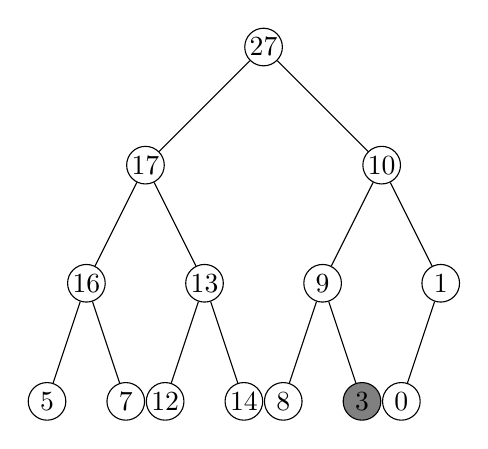
\begin{tikzpicture}[level/.style={sibling distance=30mm/#1},
treenode/.style={align=center, inner sep=0pt, text width=1.2em, text centered},
current/.style={fill=gray}]
    \node [circle,draw,treenode] {27}
      child {
        node [circle,draw,treenode] {17}
        child {
            node [circle,draw,treenode] {16}
            child {
                node [circle,draw,treenode] {5}
            }
            child {
                node [circle,draw,treenode] {7}
            }}
        child {
            node [circle,draw,treenode] {13}
            child {
                node [circle,draw,treenode] {12}
            }
            child {
                node [circle,draw,treenode] {14}
            }
        }
      }
      child {
        node [circle,draw,treenode] {10}
        child {
            node [circle,draw,treenode] {9}
            child {
                node [circle,draw,treenode] {8}
            }
            child {
                node [circle,draw,treenode,current] {3}
            }
        }
        child {
            node [circle,draw,treenode]  {1}
            child {
                node [circle,draw,treenode] {0}
            }
            child [missing]
        }
    };
    \end{tikzpicture}
\end{document}